Nowadays seismic hazard analysis serves different needs coming 
from a variety of users and applications. 
%
These may encompass engineering design, assessment of earthquake risk 
to portfolios of assets within the insurance and reinsurance sectors, 
engineering seismological research, and effective mitigation via public 
policy in the form of urban zoning and building design code formulation.

Decisions based on seismic hazard results may have impacts on
population, properties and capitals possibly with important repercussions 
on our day-to-day life. For these reasons, it is recommendable that 
the generation of hazard models and their calculation is based on 
well-recognized, state-of-the-art and tested techniques, requirements 
that must be reconciled with the need to regularly incorporate 
the most recent scientific advance. 
%
The features described below contribute to fulfill these requirements: 
%
\begin{itemize}
\item software should have have a modular and flexible structure to 
incorporate new features and offer the most recent and advanced 
techniques;
\item software should have and extensive test coverage which captures 
possible errors and avoids regressions (i.e. unexpected behaviors 
introduced by new features).
\end{itemize}
% . . . . . . . . . . . . . . . . . . . . . . . . . . . . . . . . . . . > Figure
\begin{figure}[!ht]
\centering
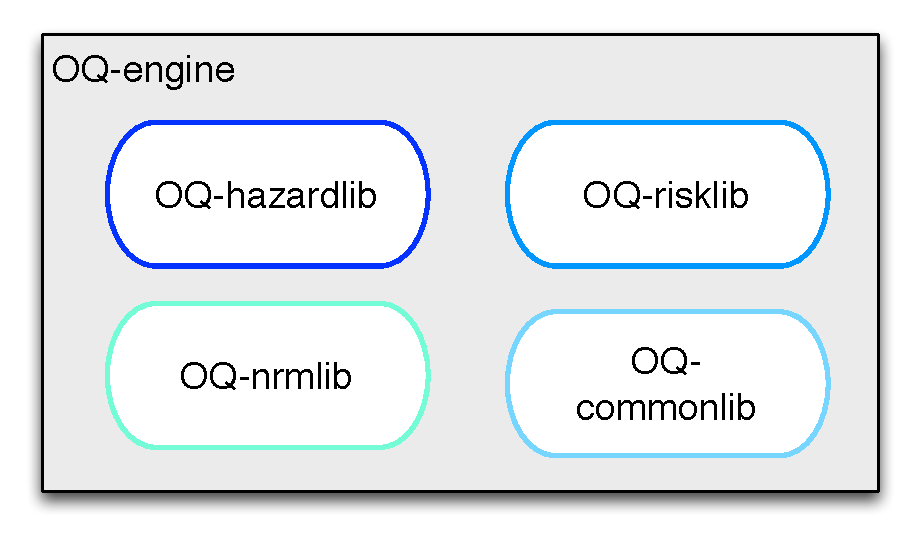
\includegraphics[width=9cm]{./Pictures/qa/oq-engine_structure.pdf}
\caption{A schematic describing the main components of the OpenQuake-engine 
    structure.}
\label{fig:oqe_structure}
\end{figure}
% . . . . . . . . . . . . . . . . . . . . . . . . . . . . . . . . . . . < Figure

In very general terms, modularity is the level to which a component 
of a system can be moved, replaced or reused. 
%
In software design modularity means the separation of the software
into smaller independent components that can be implemented, maintained 
and tested more easily and efficiently.
% 
The \gls{acr:oqe} is organized into different levels of modularity. The first
is the one separates the engine itself into a number of 
libraries (see Figure \ref{fig:oqe_structure} each one containing well 
identified knowledge, objects and methods (e.g. the OQ-hazardlib  
includes objects and methods needed to compute probabilistic 
seismic hazard). 

According to \textcite{berkes2012} the main requirements for 
scientific programming are:
\begin{itemize}
\item Error proof
\item Flexible and able to accommodate different methods
\item Reproducible and re-usable. 
\end{itemize}

The current document describes the testing procedures adopted in 
the development of the hazard component of the \gls{acr:oqe}, the 
open source hazard and risk software developed by the Global 
Earthquake Model initiative.

Software testing \parencite{myers2012} is an important, complex and 
vast discipline which develops methods and processes aimed at 
establishing that a computer code behaves according to the original 
design and user specifications. 
 
%spewhat it was designed to do and that it does not do anything unintended. Software should be predictable and consistent, offering no surprises to users. In this book we will look at many approaches to achieving this goal. 

% http://www.planit.net.au/resource/software-quality-assurance-is-it-the-same-as-testing/)
%
% ..............................................................................
\section{Testing}
Software testing can be implemented at different stages of the development 
process, clearly this implies different strategies to approach the problem.
%
The \gls{acr:oqe} and the associated libraries are developed following an 
agile paradigm. This development strategy is organized in such a way that 
the preparation of the real code is completed in parallel and fully 
integrated with the software testing process.

The software engineering community provides a wide range of testing levels
and typologies. In the current document we consider just a portion of them
with the specific intent to illustrate what has been adopted in the 
development of the \gls{acr:oqe} and particularly of its hazard component.
%
% ..............................................................................
\section{Quality Assurance}
From the IEEE ``Standard for Software Quality Assurance Processes'':
\emph{Software quality assurance is a set of activities that define and 
assess the adequacy of software processes to provide evidence that establishes 
confidence that the software processes are appropriate for and produce 
software products of suitable quality for their intended purposes. 
A key attribute of SQA is the objectivity of the SQA function with 
respect to the project. The SQA function may also be organizationally 
independent of the project; that is, free from technical, managerial, 
and financial pressures from the project.}
%
% ..............................................................................
\section{Document structure}
The document is organized into three main chapter plus and introductory 
section. 
 
The current chapter we provides a general introduction to software 
testing with a focus on the testing of scientific software. 
 
In the second chapter we describe the module, or unit, testing 
and the acceptance tests adopted and we discuss some examples. 
 
In the third and fourth chapters we describe tests where we compare 
the results computed with the \gls{acr:oqe} against the ones 
computed using different probabilistic seismic hazard analysis software.
  
Appendix \ref{sec:app1} provides details on the PEER tests 
implemented in the \gls{acr:oqhl}.
